\begin{figure}[!htbp]\centering
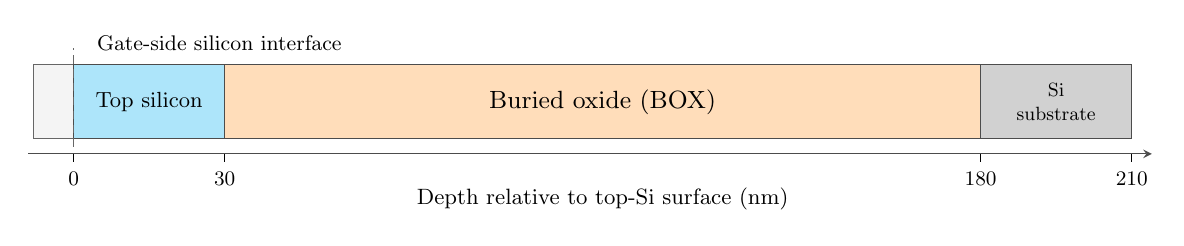
\begin{tikzpicture}[x=.064cm,y=1cm,font=\small]
  % The bar widths follow genuine SProcess 1D X-coordinate interfaces.
  \draw[fill=gray!9,draw=black!60] (-8,.5) rectangle (0,1.44);
  \draw[fill=cyan!32,draw=black!70] (0,.5) rectangle (30,1.44);
  \draw[fill=orange!27,draw=black!70] (30,.5) rectangle (180,1.44);
  \draw[fill=gray!36,draw=black!70] (180,.5) rectangle (210,1.44);
  \node[align=center,scale=.88] at (15,.97) {Top silicon};
  \node[align=center] at (105,.97) {Buried oxide (BOX)};
  \node[align=center,scale=.77] at (195,.97) {Si\\substrate};
  \draw[densely dashed,black!60] (0,.4)--(0,1.65);
  \node[anchor=west,scale=.85] at (3,1.72) {Gate-side silicon interface};
  \draw[-stealth,black!70] (-9,.31)--(214,.31);
  \foreach \xx/\lab in {0/0,30/30,180/180,210/210}{
     \draw (\xx,.31)--(\xx,.21);
     \node[anchor=north,scale=.83] at (\xx,.18) {\lab};
  }
  \node[scale=.89] at (105,-.26) {Depth relative to top-Si surface (nm)};
\end{tikzpicture}
\caption{Initial SOI material regions reconstructed from the original
one-dimensional SProcess output
\texttt{soi\_00\_start\_fps.tdr} (not a two-dimensional device
cross-section). Region-interface coordinates are
$X=-0.18000001,-0.15000001,$ and $0\,\mu$m. The 30-nm top
silicon is separated from the silicon substrate by a 150-nm
buried oxide (BOX). The diagram is an accurately scaled,
source-derived material-depth map, not a screen capture.}
\label{fig:initial_soi_material_profile}
\end{figure}
